\begin{ledgroupsized}[r]{120mm}
\footnotesize
\pstart
\noindent\textbf{Überlieferung:}
\pend
\end{ledgroupsized}
\begin{ledgroupsized}[r]{114mm}
\footnotesize
\pstart \parindent -6mm
\makebox[6mm][l]{\textit{L}}%
Konzept:
LH~XXXV~13, 3~Bl.~237\textendash238. 
Ein Bogen~2\textsuperscript{o};
Wasserzeichen		%
in Bl.~237.
Zwei Seiten auf Bl.~237~r\textsuperscript{o} und Bl.~238~v\textsuperscript{o}; 
Bl.~237~v\textsuperscript{o} und Bl.~238~r\textsuperscript{o} leer.
\pend
\end{ledgroupsized}
\vspace{5mm}
\begin{ledgroup}
\footnotesize
\pstart
\noindent%
\textbf{Datierungsgründe:} %
Das Wasserzeichen im Träger von N.\;\ref{58297} ist bislang für den Zeitraum August 1697 bis April 1703 (besonders häufig ab 1700) belegt. %
\pend
\end{ledgroup}
\selectlanguage{latin}

\vspace{8mm}
\pstart%
\normalsize%
\noindent%
\href{\Scan{LH_35_13_03_237r}}%
{\lbrack237~r\textsuperscript{o}\rbrack}\
Supponamus corpus motum 
\edtext{incurrens\indexS{incursus centralis et normalis} centraliter et normaliter}{\lemma{incurrens}\Bfootnote{%
\textit{(1)}~directe 
\textit{(2)}~centraliter et normaliter~\textit{L}}} 
in aequale quiescens\indexS{corpus incurrens centraliter et normaliter in quiescens} dare 
\edtext{ei suam velocitatem,}{\lemma{ei}\Bfootnote{%
\textit{(1)}~suum motum 
\textit{(2)}~suam velocitatem,~\textit{L}}}
et quiescere ejus loco, nec referre, quae sit figura corporis 
\edlabel{35_13_03_237-238_7a}%
\edtext{}{%
{\xxref%
{35_13_03_237-238_7a}{35_13_03_237-238_7b}}%
\lemma{alterutrius.}%
\Bfootnote{%
\textit{(1)}~Sit jam corpus 
\textit{(2)}~Sint jam 
\textit{(3)}~Ponamus jam corpus \textit{A}~\textit{L}}}%
alterutrius.
\pend
\begin{edfigure}[1em]%
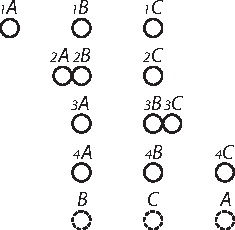
\includegraphics[scale=1]{gesamttex/edit_VIII-4/images/LH_35_13_03_237-238_d1_237r.pdf}
\edcaption{%
\edtext{\lbrack\textit{Fig.~1}\rbrack}{%
\lemma{\lbrack\textit{Fig.~1}\rbrack}%
\Cfootnote[nonum]{%
Zwei gestrichene Entwürfe zum Diagramm werden nicht wiedergegeben.}}}
\end{edfigure}
\pstart
Ponamus jam corpus \textit{A}%
\edlabel{35_13_03_237-238_7b}
incurrens in 
\edtext{aequale}{\lemma{}\Bfootnote{%
aequale \textit{erg.~L}}} 
corpus\indexS{corpus incurrens in aequale} \textit{B} ejus loco quiescere, 
et ipsi dare suum motum, corpus autem \textit{B}, pergens incurrere
\edtext{in corpus aequale \textit{C} et rursus quiescere eique}{\lemma{in corpus}\Bfootnote{%
\bars{aequale \textit{erg.}} \textit{C} 
\textit{(1)}~eique rurs 
\textit{(2)}~et rursus quiescere eique~\textit{L}}} 
dare suum motum; manifestum est quid 
\edlabel{35_13_03_237-238_1a}%
\edtext{}{{\xxref{35_13_03_237-238_1a}{35_13_03_237-238_1b}}%
\lemma{eveniat}\Bfootnote{%
\textit{(1)}~, sed quid si fingamus dum corpora \textit{B} et \textit{C} sejungi debent, \textit{B} quiescente, et \textit{C} pergente supervenire causam quae ea sejungi vetet, dicemus 
\textit{(2)}~. Et idem est~\textit{L}}}%
eveniat.
\pend
\pstart
Et idem est\edlabel{35_13_03_237-238_1b}
etsi sint corpora quotcunque \textit{A}, \textit{B}, \textit{C}, \textit{D}, ut semper fiat 
permutatio,\indexS{permutatio celeritatis} et cum ante 
concursum\indexS{concursus} omnem, moveatur tantum \textit{A}, quiescentibus 
\textit{B}, \textit{C}, \textit{D}, post omnem concursum\indexS{concursus} movebitur 
tantum \textit{D}, quiescentibus \textit{A}, \textit{B}, \textit{C}, perinde ac si \textit{A} ipsa \textit{B}, \textit{C}, 
\textit{D}, potuisset penetrare,\indexS{penetratio} et motum suum quasi ipsis non obstantibus continuasset, neque enim differunt 
status quarti momenti verus, a ficto per puncta designato, qui prodiisset, si \textit{A} transiisset et penetrando. \pend
\pstart Cumque idem
\edtext{prodeat etsi corpora}{\lemma{prodeat etsi}\Bfootnote{%
\textit{(1)}~puncta 
\textit{(2)}~corpora~\textit{L}}} 
\textit{A}, \textit{B}, \textit{C}, sibi immediata ponantur, seu etsi distantia 
\edtext{evanescat. Hinc}{\lemma{evanescat}\Bfootnote{%
\textit{(1)}~, generaliter apparet quis sit motus 
\textit{(2)}~. Hinc~\textit{L}}} 
si corpus incurrat\indexS{corpus incurrens in plura aequalia} simul in 
\edtext{plura aequalia in eadem}{\lemma{plura}\Bfootnote{%
\textit{(1)}~in ea 
\textit{(2)}~aequalia in eadem~\textit{L}}} 
linea posita, sic ut omnia centraliter et directe
\edtext{in se niti posse}{\lemma{in se}\Bfootnote{%
\textit{(1)}~incurrere 
\textit{(2)}~niti posse intelligantur,
\textit{(a)}~qui
\textit{(b)}~vel~\textit{L}}} 
etiam si plura incurrant\indexS{corpora plura incurrentia in plura alia} in 
\edtext{alia}{\lemma{}\Bfootnote{%
alia \textit{erg.~L}}} 
plura quiescentia, 
semper idem
fore ac si corpora se penetrarent,\indexS{penetratio} seu sibi non 
\edtext{obstarent. Quod}{\lemma{obstarent.}\Bfootnote{%
\textit{(1)}~Nam 
\textit{(2)}~Ea 
\textit{(3)}~Quod~\textit{L}}} 
demonstrari potest, tum ex hypothesi communis motus\indexS{motus communis} nihil 
mutantis,\indexS{hypothesis motus communis nihil mutantis} 
tum etiam si singulatim concurrere facias corpus corpori aequali sine ullo 
contactu.
\pend
\begin{edfigure}[1em][0.5em]    	%
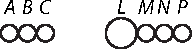
\includegraphics[scale=1]{gesamttex/edit_VIII-4/images/LH_35_13_03_237-238_d2_237r.pdf}
\edcaption[0.25em]{\edtext{\lbrack\textit{Fig.~2}\rbrack}{%
\lemma{\lbrack\textit{Fig.~2}\rbrack}%
\Cfootnote[nonum]{%
Ein gestrichener Entwurf zum Diagramm wird nicht wiedergegeben.}}}
\end{edfigure}
\pstart 
Quid si jam corpora aequalia et inaequalia misceamus, 
\edtext{ut si tres globos\indexS{globus}}{\lemma{ut}\Bfootnote{%
\textit{(1)}~si corpora 
\textit{(2)}~si tres globos~\textit{L}}} 
\textit{ABC}, occurrere faciamus in quatuor globos\indexS{globus} \textit{LMNP}, ex quibus \textit{L} sit major, sed \textit{MNP}, ipsis \textit{ABC} aequales, an concludere licebit ex 
\edtext{principio aequivalentiae\indexS{principium aequivalentiae} ad penetrationem\indexS{penetratio}}{\lemma{principio}\Bfootnote{%
\textit{(1)}~penetrationis
\textit{(2)}~aequivalentiae ad penetrationem~\textit{L}}} 
quiescere \textit{ABC}, pergere 
\edlabel{35_13_03_237-238_2a}%
\edtext{}{{\xxref{35_13_03_237-238_2a}{35_13_03_237-238_2b}}%
\lemma{\textit{MNP}.}\Bfootnote{%
\textit{(1)}~Hoc 
\textit{(a)}~demo 
\textit{(b)}~verum demonstrabitur ex hoc 
\textit{(2)}~An hoc 
\textit{(3)}~Videamus~\textit{L}}}%
\textit{MNP}.
\pend
\begin{edfigure}[1em][0.75em]		%
\hfill
\includegraphics[scale=1]{%
gesamttex/edit_VIII-4/images/LH_35_13_03_237-238_d3_237r.pdf%
}%
\hfill%
\includegraphics[scale=1]{%
gesamttex/edit_VIII-4/images/LH_35_13_03_237-238_d4_237r.pdf%
}
\hfill
\edcaption{%
\lbrack\textit{Fig.~3}\rbrack \hspace*{42mm}
\lbrack\textit{Fig.~4}\rbrack}
\end{edfigure}
\pstart 
Videamus\edlabel{35_13_03_237-238_2b}
an hoc verum demonstretur ex hoc
principio, quod corpore $\aleph$ 
\edtext{incurrente in corpus $\beth$}{\lemma{incurrente in}\Bfootnote{%
\textit{(1)}~murum 
\textit{(2)}~corpus $\beth$~\textit{L}}} 
utcunque, et corpore $\beth$ incurrente in murum\indexS{incursus in murum}
non cedentem $\gimel$, atque inde ea qua venit vi 
\edtext{repercusso, ac cum corpore $\aleph$}{\lemma{repercusso,}\Bfootnote{%
\textit{(1)}~debeant omnia
\textit{(2)}~ac corpus $\aleph$ 
\textit{(3)}~ac cum corpore $\aleph$~\textit{L}}} 
rursus concurrente, debeat redire status prior. Itaque si corpus $\aleph$ pergit post 
\edtext{incursum, at}{%
\lemma{incursum,}%
\Bfootnote{%
\textit{(1)}~cum %
\textit{(2)}~ut~\textit{L}}}
si $\beth$
\edtext{quiescente $\aleph$}{%
\lemma{quiescente}%
\Bfootnote{%
\textit{(1)}~$\beth$ si %
\textit{(2)}~$\aleph$~\textit{L}}}
sit majus, sufficit repercuti $\beth$ a muro, sin $\aleph$ sit minus
\edtext{et regrediatur,}{%
\lemma{et}\Bfootnote{%
\textit{(1)}~repercuti
\textit{(2)}~regrediatur%
~\textit{L}}}
oportet ipsi quoque opponi murum $\daleth$, ut repercussu iterum 
concurrant, sed nullo opus muro, si corpora $\aleph$ et $\beth$ moveantur circa centrum\indexS{motus circa centrum} \hebr{h}. 
Ita enim post concursum\indexS{concursus} a contraria parte circuli veniendo rursus
\edlabel{35_13_03_237-238_3a}%
\edtext{}{{\xxref{35_13_03_237-238_3a}{35_13_03_237-238_3b}}%
\lemma{concurrent.}\Bfootnote{%
\textit{(1)}~Hoc principio posito patet corpus
\textit{(a)}~qui
\textit{(b)}~$\aleph$ \bars{incurrens \textit{streicht Hrsg.}} in qui
\textit{(2)}~Sed video aliud potius esse principium, ut si 
\bars{corpus $\aleph$ incurrat \textit{streicht Hrsg.}} in corpus $\beth$
\textit{(3)}~Sed video tale principium%
~\textit{L}}}%
concurrent.
\pend
\pstart 
Sed video tale principium\edlabel{35_13_03_237-238_3b}
hic non satis applicari potest, et illud tamen manifestum est, si \textit{ABC} aequetur ipsi \textit{L} majori, 
locum habere quasi penetrationem,\indexS{penetratio} item si loco \textit{L}, 
essent duo \textit{H} et \textit{L} vel
\edtext{plura quorum quodlibet aequale ipsis \textit{ABC} simul.}{%
\lemma{plura}\Bfootnote{%
\textit{(1)}~simul aequalia ipsi
\textit{(2)}~quorum \lbrack...\rbrack\ simul.%
~\textit{L}}}
\pend
\pstart%
Haec ultra 
\edlabel{35_13_03_237-238_4a}%
\edtext{}{{\xxref{35_13_03_237-238_4a}{35_13_03_237-238_4b}}%
\lemma{prosequenda.}%
\Bfootnote{%
\textit{(1)}~Elegans etiam
\textit{(a)}~hoc principium
\textit{(b)}~talis meth
\textit{(2)}~Si corpus unum
\textit{(a)}~\bars{in \textit{streicht Hrsg.}} corpora composita simul occurrat,
\textit{(b)}~in corporum compositum
\textit{(aa)}~incurrat
\textit{(bb)}~quiescens sibi aequale occurrat%
~\textit{L}}}%
prosequenda.%
\pend%
\begin{edfigure}[0.5em][0.75em]    	%
\includegraphics[scale=1]{%
gesamttex/edit_VIII-4/images/LH_35_13_03_237-238_d5_237r.pdf}
\edcaption[0.25em]{\lbrack\textit{Fig.~5, gestr.}\rbrack}
\end{edfigure}
\pstart 
Si corpus unum in corporum compositum quiescens sibi aequale occurrat,\indexS{corpus in quiescens aequale occurrens}%
\edlabel{35_13_03_237-238_4b}
motum suum ipsis
\edtext{dabit. Non juvat ad methodum.}{%
\lemma{dabit.}\Bfootnote{%
\textit{(1)}~Sed praestat tamen
\textit{(a)}~corpus in plura \bars{occurrens \textit{streicht Hrsg.}} sibi
\textit{(b)}~ex com
\textit{(c)}~haec meth
\textit{(2)}~Sed quia
\textit{(a)}~non juvat ad methodum praestat hoc modo \bars{rem \textit{streicht Hrsg.}} 
duci ex principio penetrationis.
\textit{(3)}~Non juvat ad methodum.%
~\textit{L}}}
\pend
\pstart
\href{\Scan{LH_35_13_03_238v}}%
{\lbrack238~v\textsuperscript{o}\rbrack}
Si duo 
\edtext{corpora aequalia\indexS{corpora aequalia} aequal\lbrack i\rbrack\ motu\indexS{motus aequalis}}{%
\lemma{corpora}%
\Bfootnote{%
\textit{(1)}~aequali motu %
\textit{(2)}~aequalia \bars{aequalia \textit{ändert Hrsg.}} motu~\textit{L}}}
ferantur, et concurrant, quod non nisi contrario motu fieri 
\edtext{potest, ponamus}{\lemma{potest,}\Bfootnote{%
\textit{(1)}~erit 
\textit{(2)}~ponamus~\textit{L}}} 
pro 
\edtext{fundamento ambo}{\lemma{fundamento}\Bfootnote{%
\textit{(1)}~ipsa 
\textit{(2)}~ambo~\textit{L}}} 
reflecti eo motu quo venere. 
\pend
\begin{edfigure}%
\includegraphics[scale=1]{%
gesamttex/edit_VIII-4/images/LH_35_13_03_237-238_d6_238v.pdf}
\edcaption{\edtext{\lbrack\textit{Fig.~6}\rbrack}{%
\lemma{\lbrack\textit{Fig.~6}\rbrack}%
\Cfootnote[nonum]{Ein gestrichener Entwurf zum Diagramm wird nicht wiedergegeben.}}}
\end{edfigure}
\pstart 
Si jam duo corpora inaequalia\indexS{corpora inaequalia} concurrant motu aequali,\indexS{motus aequalis} 
dividamus in partes aequales, ut si \textit{A}, \textit{B}, incurrant in \textit{C} fit inversum prioris, seu quasi 
\edlabel{35_13_03_237-238_6a}%
\edtext{}{%
{\xxref%
{35_13_03_237-238_6a}{35_13_03_237-238_6b}}%
\lemma{penetratio.}\Bfootnote{%
\textit{(1)}~Ut fieret etsi motus esset inaequales. 
\textit{(2)}~Videamus~\textit{L}}}%
penetratio.\indexS{penetratio}%
\pend
\pstart
Videamus%
\edlabel{35_13_03_237-238_6b}
an idem demonstrari possit etsi ferantur motu 
inaequali.\indexS{motus inaequalis} Sint duo 
\edtext{corpora aequalia\indexS{corpora aequalia} \textit{A} et \textit{B}}{\lemma{corpora}\Bfootnote{%
\textit{(1)}~\textit{A} et \textit{B} 
\bars{aequalia \textit{erg.}} concurrentia 
\textit{(2)}~aequalia \textit{A} et \textit{B} concurrentia~\textit{L}}} 
motu inaequali,\indexS{motus inaequalis} dividamus motum 
\edtext{inaequalem in}{\lemma{inaequalem}\Bfootnote{%
\textit{(1)}~,~et 
\textit{(2)}~in~\textit{L}}} 
aequales interruptos.\indexS{motus aequales interrupti} Et primum 
\edtext{sit motus}{%
\lemma{sit}%
\Bfootnote{%
\textit{(1)}~unus %
\textit{(2)}~motus~\textit{L}}}
ipsius \textit{A} duplus ipsius \textit{B} simplus. Primum corpus \textit{A}, et corpus \textit{B} concurrant motu 
\edtext{aequali.\indexS{motus aequalis} Et hoc}{\lemma{aequali}\Bfootnote{%
\textit{(1)}~, reflectentur ambo motu
\textit{(a)}~comm
\textit{(b)}~quo venere, 
\raisebox{-0.3ex}{
\includegraphics[scale=1]{gesamttex/edit_VIII-4/images/LH_35_13_03_237-238_d7_238v.pdf}} \enskip\lbrack\textit{Fig.~7}\rbrack\nobreak\enskip\nobreak 
sed praeterea 
\textit{(2)}~. Et hoc~\textit{L}}} 
fiat uno minuto, accipiet utrumque conatum recedendi\indexS{conatus recedendi} 
ea vi qua venit. Sed hunc conatum servabimus, et 
\edtext{jam adhibeamus}{\lemma{jam}\Bfootnote{%
\textit{(1)}~praeterea 
\textit{(2)}~ponamus 
\textit{(3)}~adhibeamus~\textit{L}}} 
intervallum, quo \textit{A} movetur et \textit{B} quiescit, hoc casu \textit{A} dat suum motum ipsi \textit{B}, 
et \textit{A} quiescet, ac \textit{B} accipiat conatum 
novum simplum celeritatis, qui additus priori, faciet ut \textit{B} accipiat duos gradus 
velocitatis et \textit{A} habeat unum. 
Itaque hac ratione, si motus 
\edtext{sunt aequales,\indexS{motus aequales}}{\lemma{sunt}\Bfootnote{%
\textit{(1)}~aequabiles 
\textit{(2)}~aequales,~\textit{L}}} 
demonstrabitur permutatio 
\edtext{celeritatis,\indexS{permutatio celeritatis} positis his duabus}{\lemma{celeritatis,}\Bfootnote{%
\textit{(1)}~ex eo quo 
\textit{(2)}~positis 
\textit{(a)}~duobus 
\textit{(aa)}~cor
\textit{(bb)}~principi
\textit{(b)}~corpora duo aequalia 
\textit{(c)}~his duabus~\textit{L}}} 
regulis, quod duo corpora aequalia aequalibus 
\edtext{celeritatibus concurrentia\indexS{corpora aequalia aequalibus celeritatibus concurrentia} iisdem}{\lemma{celeritatibus}\Bfootnote{%
\textit{(1)}~mota iisd 
\textit{(2)}~concurrentia iisdem~\textit{L}}} 
repercutiantur, et quod corpus motum det suum motum aequali 
\edlabel{35_13_03_237-238_9a}%
\edtext{}{%
{\xxref%
{35_13_03_237-238_9a}{35_13_03_237-238_9b}}%
\lemma{quiescenti}\Bfootnote{%
\textit{(1)}~. Hunc se 
\textit{(2)}~; accedente 
\textit{(a)}~meth 
\textit{(b)}~fictione interruptionis 
\textit{(aa)}~qua 
\textit{(bb)}~qua 
\textit{(cc)}~quemadmodum~\textit{L}}}%
quiescenti; accedente fictione interruptionis\indexS{fictio interruptionis} 
\edtext{quemadmodum\edlabel{35_13_03_237-238_9b} volebant quidam veteres\indexS{veteres}
motus inaequalitatem\indexS{inaequalitas motus} esse a interpositis
\edlabel{35_13_03_237-238_10a}%
\edtext{}{%
{\xxref%
{35_13_03_237-238_10a}{35_13_03_237-238_10b}}%
\lemma{quietulis.}\Bfootnote{%
\textit{(1)}~Unde et res 
\textit{(2)}~Unde alternantia 
\textit{(a)}~moment 
\textit{(b)}~temporis intervalla~\textit{L}}}%
quietulis.\indexS{quietula interposita}}{%
\lemma{quemadmodum \lbrack...\rbrack\ quietulis}%
\Cfootnote{%
Gemeint ist \indexN{\textls{Empedokles} von Agrigent um 430 v. Chr.}Empedokles, 
dem Leibniz an mehreren Orten diese Ansicht zuschreibt (siehe bspw. \cite{02144}\textit{Pacidius Philalethi}, in \textit{LSB} VI~3, S.\;542 Z.\;5\,f.). 
Damit folgt er wohl \indexN{\textls{Aristoteles} 384\textendash322 v. Chr.}Aristoteles, 
\cite{00235}\textit{Physica} VIII\;1, 252\,a\;5--10 (= \cite{02145}\textsc{Diels/Kranz}, \textit{Die Fragmente der Vorsokratiker}, 9. Aufl. Berlin 1960, 31 A 38, Bd.\;I, S.\,290).}}
Unde alternantia temporis intervalla\indexS{intervalla temporis alternantia}%
\edlabel{35_13_03_237-238_10b}
sumenda essent etiam pro resultatis, 
\edtext{seu inpressis conatibus unoquoque}{\lemma{seu}\Bfootnote{%
\textit{(1)}~concursibus
\textit{(2)}~inpressis 
\textit{(a)}~, uno 
\textit{(b)}~conatibus unoquoque~\textit{L}}} 
valente pro sua alternatione 
\edtext{sic\lbrack:\rbrack\ \textit{A} habet duos gradus velocitatis,}{\lemma{sic}\Bfootnote{%
\textit{(1)}~\textit{A} 
\textit{(a)}~in
\textit{(b)}~incurrit \bars{in \textit{erg.}} \textit{B} minuto 3
\textit{(aa)}~et minuto
\textit{(bb)}~\textit{A} concurrit cum \textit{B} minuto 1. 
\textit{(cc)}~et \textit{A} incurrit 
\textit{(aaa)}~et dat
\textit{(bbb)}~et accipit motum 
\textit{(2)}~\textit{A} habet duos gradus velocitatis,~\textit{L}}} 
et \textit{B} unum. Ponatur tempus dividi in minuta 
\edtext{1, 2, 3, 4, etc.}{%
\lemma{}%
\Bfootnote{%
1, 2, 3, 4, \bars{5, 6. \textit{gestr.}} etc.~\textit{L}}}
Et minuta 1, 3, 5 esse pro gradu velocitatis uno in \textit{A}, et uno 
\edtext{in \textit{B}, et eo quod inde provenit, sed minuta 2, 4, 6, etc.}{\lemma{in \textit{B},}\Bfootnote{%
\textit{(1)}~sed 
\textit{(a)}~minutum 2 
\textit{(b)}~minuta 
\textit{(2)}~et \lbrack...\rbrack\  2, 4, 6, etc.~\textit{L}}} 
esse pro altero gradu velocitatis in \textit{A}, 
et pro quiete in \textit{B}, et quod inde provenit.
\edtext{Minuto 1, concurrunt}{%
\lemma{Minuto 1,}%
\Bfootnote{%
\textit{(1)}~concurrit %
\textit{(2)}~concurrunt~\textit{L}}}
\textit{A} et \textit{B} celeritate unius gradus, et ideo minuto 3 regredietur \textit{A} celeritate unius gradus, 
et regredietur et \textit{B} celeritate unius gradus. 
Minuto 2 \textit{A} celeritate unius gradus incurret in \textit{B} quiescens, 
et ideo pro minuto 4 quiescet 
\edtext{\textit{A}, et regredietur}{\lemma{\textit{A}, et}\Bfootnote{%
\textit{(1)}~progredietur 
\textit{(2)}~regredietur~\textit{L}}} 
\textit{B} celeritate unius gradus. 
Hinc quia minuto 3 regredietur \textit{A} celeritate unius gradus, et minuto 4, quiescet, 
sed minuto 3 regredietur \textit{B} celeritate unius gradus, 
et minuto 
\edtext{\lbrack4\rbrack}{%
\lemma{}%
\Bfootnote{%
3 \textit{L ändert Hrsg.}}}
etiam,
\edtext{patet velocitates ipsius \textit{A} et \textit{B} fuisse permutat\lbrack a\rbrack s, in cujusque regressu,\indexS{regressus}}{\lemma{patet}\Bfootnote{%
\textit{(1)}~ce 
\textit{(2)}~jungendo in unum haec 
\textit{(3)}~is 
\textit{(4)}~statum qui fuit ipsius \textit{A} 
\textit{(5)}~status ipsius \textit{A} et \textit{B} fuisse permutatos 
\textit{(6)}~velocitates ipsius \textit{A} et \textit{B} fuisse \bars{permutatos \textit{ändert Hrsg.}} , in
\textit{(a)}~regr
\textit{(b)}~cujusque regressu~\textit{L}}} 
et locum habere quasi 
\edlabel{35_13_03_237-238_5a}%
\edtext{}{{\xxref{35_13_03_237-238_5a}{35_13_03_237-238_5b}}%
\lemma{penetrationem.}\Bfootnote{%
\textit{(1)}~Ope hypotheseos
\textit{(2)}~Ope harum 
\textit{(a)}~trium hypothesium: quod co 
\textit{(b)}~duarum hypothesium~\textit{L}}}%
penetrationem.\indexS{penetratio}
\pend
\pstart 
Ope harum duarum hypothesium\lbrack,\rbrack%
\edlabel{35_13_03_237-238_5b}
quod duo corpora 
\edtext{celerita\lbrack te\rbrack s}{\lemma{}\Bfootnote{%
celeritas \textit{L ändert Hrsg.}}} 
habentia molibus reciprocas\indexS{celeritates molibus reciprocae} redeant suo 
\edtext{motu (\protect\vphantom)unde}{%
\lemma{motu}%
\Bfootnote{%
\textit{(1)}~et %
\textit{(2)}~(\protect\vphantom)unde~\textit{L}}}
et sequitur aequalia aequalibus concurrentia suo motu 
\edtext{redire\protect\vphantom() et quod habeatur casus corporis incurrentis in quiescens\lbrack,\rbrack\indexS{corpus incurrens in quiescens}}{\lemma{redire\protect\vphantom() et}\Bfootnote{%
\textit{(1)}~ex 
\textit{(a)}~eo quod corpus incurrens in aequale quiescens ei dat suum motum, 
vel generalius quod in \bars{corporibus \textit{erg.}} aequalibus locum habeat quasi penetratio,
\textit{(b)}~\bars{motu quem \textit{streicht Hrsg.}} corpus 
\textit{(2)}~quod habeatur 
\textit{(a)}~motus quem corpus incurrens 
\textit{(b)}~casus corporis incurrentis in quiescens~\textit{L}}} 
cuncta possunt derivari in duobus 
\edtext{corporibus. Si corpus \textit{A} simplum}{\lemma{corporibus.}\Bfootnote{%
\textit{(1)}~Corpus \textit{A} sit 
\textit{(a)}~dupla velocita 
\textit{(b)}~3plo velocius quam corpus \bars{\textit{B}, et \textit{streicht Hrsg.}}
corpus \textit{B} triplo 
\textit{(aa)}~prius quam corpus \textit{A} 
\textit{(bb)}~majus quam corpus \textit{A}.
\textit{(2)}~Si corpus 
\textit{(a)}~\textit{A} velocitate 
\textit{(b)}~\textit{A} 
\textit{(aa)}~triplum 
\textit{(bb)}~simplum~\textit{L}}} 
velocitate quacunque \textit{v} incurrat 
\edtext{in corpus triplum quiescens, tunc}{\lemma{corpus}\Bfootnote{%
\textit{(1)}~simplum 
\textit{(2)}~triplum quiescens, 
\textit{(a)}~erit 
\textit{(b)}~tunc~\textit{L}}} 
\edlabel{35_13_03_237-238_8a}%
\edtext{}{%
{\xxref%
{35_13_03_237-238_8a}{35_13_03_237-238_8b}}%
\lemma{}\Afootnote{%
\textit{Am Rand}: %
\textit{vv}.\textsuperscript{\lbrack a\rbrack} $\displaystyle\frac{1}{4}vv+\displaystyle\frac{3}{4}vv$.
\\[1.5ex] %
{\footnotesize \textsuperscript{\lbrack a\rbrack} 
\textit{(1)}~$3vv$. $\displaystyle\frac{3}{4}vv+\displaystyle\frac{9}{4}vv$. 
\textit{(2)}~\textit{vv}. $\displaystyle\frac{1}{4}vv+\displaystyle\frac{3}{4}vv$.~\textit{L}}}}%
ipsius \textit{A} velocitas post ictum\indexS{ictus} erit $-\displaystyle\frac{1}{2}v$ et 
\edtext{corporis tripli}{%
\lemma{corporis}%
\Bfootnote{%
\textit{(1)}~\textit{B} %
\textit{(2)}~tripli~\textit{L}}}
\edtext{velocitas 
\rule[-2.2ex]{0pt}{5.5ex}$=\displaystyle\frac{1}{2}v$.\edlabel{35_13_03_237-238_8b}
Ponatur}{\lemma{velocitas}\Bfootnote{%
\textit{(1)}~$\displaystyle\frac{3}{4}v$.
\textit{(2)}~$=\displaystyle\frac{1}{2}v$.
\textit{(a)}~\bars{Jam \textit{streicht Hrsg.}} sint 
\textit{(aa)}~momenta 
\textit{(bb)}~minuta divisa in tres classes. Primum 
\textit{(b)}~Ponatur~\textit{L}}} 
corpus \textit{A} ut 1, habere velocitatem ut 3 et corpus \textit{B} ut 3 velocitatem ut 1. 
Dividatur tempus in tres minutorum classes, 
primo minuto \textit{A}%
\edtext{.1}{%
\lemma{}%
\Bfootnote{%
.1 %
\textit{erg.~L}}}
velocitate 
\edtext{\lbrack ut 1.\rbrack}{%
\lemma{}%
\Bfootnote{%
ut 1. %
\textit{erg.~Hrsg.}}}
concurret ipsi \textit{B}%
\edtext{.3}{%
\lemma{}%
\Bfootnote{%
.3 %
\textit{erg.~L}}}
\edtext{velocitate ut 1. et \textit{A}}{\lemma{velocitate}\Bfootnote{%
\bars{ut~\textit{erg.}}~1. 
\textit{(1)}~Ergo \textit{A} pro minuto 4 regredietur velocitate 1. et \textit{B} itidem. 
Secundo minuto \textit{A} velocitate ut 1, incurret ipsi \textit{B}.3, quiescenti
et ipsius \textit{A} velocitas 
\textit{(a)}~erit
\textit{(b)}~regrediendi 
\textit{(2)}~et \textit{A}~\textit{L}}} 
pro minuto 4 regredietur velocitate $-h$, et \textit{B} velocitate $-\pi$ perget. 
Minuto secundo
\textit{A}. velocitate ut 1. incurret in \textit{B}. quiescens, et \textit{A} regredietur
\edtext{pro minuto 5}{%
\lemma{}%
\Bfootnote{%
pro minuto 5 %
\textit{erg.~L}}}
velocitate $-\displaystyle\frac{1}{2}$ 
\edtext{et \textit{B} propelletur}{\lemma{et \textit{B}}\Bfootnote{%
\textit{(1)}~progredietur 
\textit{(2)}~propelletur~\textit{L}}} 
velocitate \rule[-2.2ex]{0pt}{5.7ex}$+\displaystyle\frac{1}{2}$. Minuto 
\edtext{3\textsuperscript{tio} pro minuto 6\textsuperscript{to}}{\lemma{3\textsuperscript{tio}}\Bfootnote{%
\textit{(1)}~\textit{A}.1 velocitate ut 1. incurrat 
\textit{(2)}~pro minuto 6\textsuperscript{to}~\textit{L}}} 
fiat
\edtext{idem. Itaque}{%
\lemma{}%
\Bfootnote{%
idem \bars{pro 3~\textit{erg., streicht Hrsg.}}. Itaque~\textit{L}}}
minutis 4, 5, 6, erit velocitas ipsius \textit{A}, 
$-h-\displaystyle\frac{1}{2}-\displaystyle\frac{1}{2}=-h-1$
et velocitas ipsius \textit{B} erit 
\edtext{\lbrack$-\pi$\rbrack}{\lemma{}\Bfootnote{%
$\pi$ \textit{L ändert Hrsg.}}} 
$+\displaystyle\frac{1}{2}+\displaystyle\frac{1}{2}$\rule[-2.4ex]{0pt}{5.7ex} seu $-\pi +1$. 
Quoniam vero ex hypothesi quod \textit{A} et \textit{B} priore 
celeritate regrediuntur, debet esse $-h-1=-3$, ergo $h=2$ et $-\pi +1=1$. 
Ergo $\pi =0$. Inventa ergo sunt \textit{h} et $\pi$. 
Et ideo si \textit{A}.1, velocitate 3, concurrat ipsi \textit{B}.3, velocitate ut 1, post 
\edtext{ictum \textit{A} repercutietur}{\lemma{ictum}\Bfootnote{%
\textit{(1)}~regredientur velocitate 
\textit{(a)}~eadem qua occurrere 
\textit{(b)}~dupla ejus qua venere. Hinc \textit{A} regredietur velocitate 
\textit{(2)}~\textit{A} repercutietur~\textit{L}}} 
velocitate dupla ejus qua venit et \textit{B} quiescet. 
$x=1-3=-2=-h$ et $z=-3+1+2=0=-\pi$ quod succedit. \pend
